\section{Amazon Elastic Transcoder}
\label{sec:Amazon Elastic Transcoder}

  Amazon Elastic Transcoder lets you convert media files that you have stored in Amazon S3 into media files in the formats required by consumer playback devices. For example, you can convert large, high-quality digital media files into formats that users can play back on mobile devices, tablets, web browsers, and connected televisions.
Amazon Elastic Transcoder lets you convert media files that you have stored in Amazon Simple Storage Service (Amazon S3) into media files in the formats required by consumer playback devices. For example, you can convert large, high-quality digital media files into formats that users can play back on mobile devices, tablets, web browsers, and connected televisions.

\begin{figure}[htb] %  figure placement: here, top, bottom
 \centering
 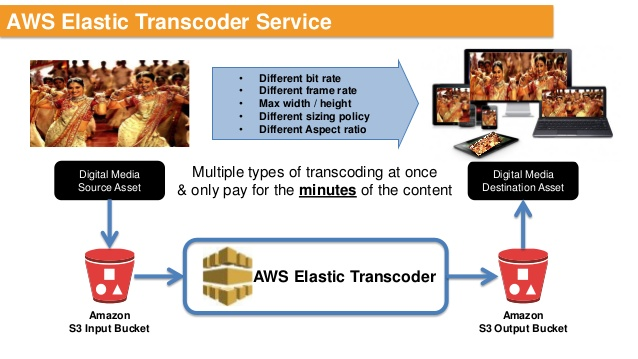
\includegraphics[width=1.0\linewidth]{images/chapter4/aws_transcoder.jpg}\hfill
 \caption[The Elastic Transcoder Lifecycle]{The Elastic Transcoder Lifecycle}
 \label{fig:fourV}
\end{figure}

Elastic Transcoder has four components:
\begin{itemize}

\item \textbf{Jobs} do the work of transcoding. Each job converts one file into up to 30 formats. For example, if you want to convert a media file into six different formats, you can create files in all six formats by creating a single job. When you create a job, you specify the name of the file that you want to transcode, the names that you want Elastic Transcoder to give to the transcoded files, and several other settings. For each format that you want to transcode into, you also specify a template, known as a preset (see below), that contains the audio and video settings that you want to use for the transcoded file or files.

\item \textbf{Pipelines} are queues that manage your transcoding jobs. When you create a job, you specify which pipeline you want to add the job to. Elastic Transcoder starts processing the jobs in a pipeline in the order in which you added them. If a pipeline already contains jobs when you create a new job, Elastic Transcoder queues the newest job and begins processing it as soon as resources are available for that pipeline. If the pipeline is already using all of its resources, Elastic Transcoder begins processing the next job in the pipeline when it finishes one of the jobs that it's currently processing. A pipeline can process more than one job simultaneously, and the time required to complete a job varies significantly based on the size of the file you're converting and the job specifications. Accordingly, jobs don't necessarily complete in the order in which you create them.You can temporarily stop processing jobs by pausing the pipeline.

\item \textbf{Presets} are templates that contain most of the settings for transcoding media files from one format to another. Elastic Transcoder includes some default presets for common formats, for example, several iPod and iPhone versions. You can also create your own presets for formats that aren't included among the default presets. You specify which preset you want to use when you create a job.


\begin{figure}[htbp] %  figure placement: here, top, bottom
 \centering
 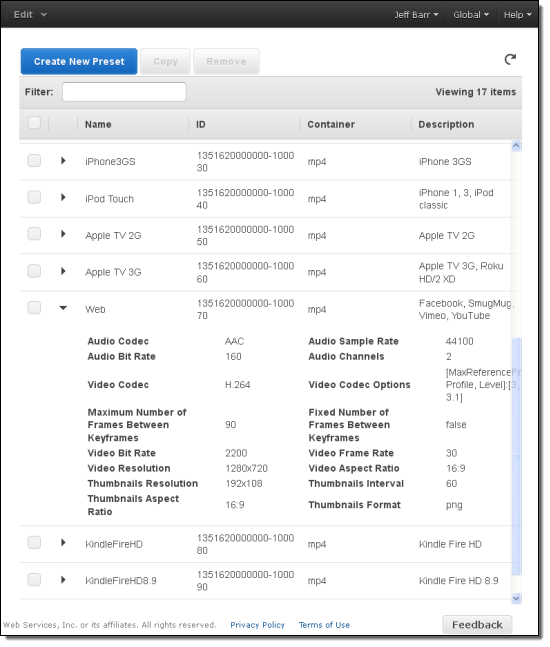
\includegraphics[width=1.0\linewidth]{images/chapter4/aws_transcoder1.png}\hfill
 \caption[Example of Preset]{Example of Preset}
 \label{fig:fourV}
\end{figure}


\item \textbf{Notifications} let you optionally configure Elastic Transcoder and Amazon Simple Notification Service to keep you apprised of the status of a job: when Elastic Transcoder starts processing the job, when Elastic Transcoder finishes the job, and whether Elastic Transcoder encounters warning or error conditions during processing. Notifications eliminate the need for polling to determine when a job has finished. You configure notifications when you create a pipeline.
\end{itemize}

